\documentclass{article}
\title{Nechyba Ch.11 短期生产者模型}
\author{Dawei Wang}
\date{\today}
\usepackage{ctex}
\usepackage{amsmath}
\usepackage{amssymb}
\usepackage{graphicx} %插入图片的宏包
\usepackage{float} %设置图片浮动位置的宏包
\usepackage{subfigure} %插入多图时用子图显示的宏包
\begin{document}
	\maketitle
经济主体把劳动、原材料和土地等“投入品”组合在一起生产出“产出品”。

假定生产者只在乎利润。

\hspace*{\fill}

两种利润最大化的观点:

1.直接展示生产者如何通过选择使他们位于最高的“无差异曲线”上的生产计划来实现利润最大化;

2.假设生产者先分析他们的成本,一旦他们清楚不同的生产计划的成本,就会自动根据生产的收益来判断哪种计划会带来最大的利润。

\section{短期一种投入/一种产出模型}
\subsection{生产者面对的技术约束}

生产计划、生产者选择集与生产边界:

用技术可行条件下的生产者选择集代表生产计划集合,生产者选择集可以简单定义为在给定条件下的技术可行条件下生产者所有生产计划的集合。

\hspace*{\fill}

位于消费者选择集内的消费束意味着消费者预算有剩余未花费,这意味消费者可以做到更好。类似地,位于生产者选择集内的生产计划意味着部分投入闲置,在相同的投入水平下可以产出更多。之前将消费集的边界定义为预算约束,现在将生产集的边界定义为生产边界。只有沿着生产边界的计划才表示没有投入的浪费。因此,正如消费者尽可能选择预算线上的消费束达到最优一样,生产者尽可能选择预算线上的消费束达到最优一样,生产者尽可能选择生产边界上的生产计划。

生产边界的斜率是用增加的生产表示的额外一单位投入的边际收益。

\hspace*{\fill}

边际产出递减规律:要素的投入在现实世界里一定会出现边际产出递减。

\begin{figure}[H] %H为当前位置,!htb为忽略美学标准,htbp为浮动图形
	\centering %图片居中
	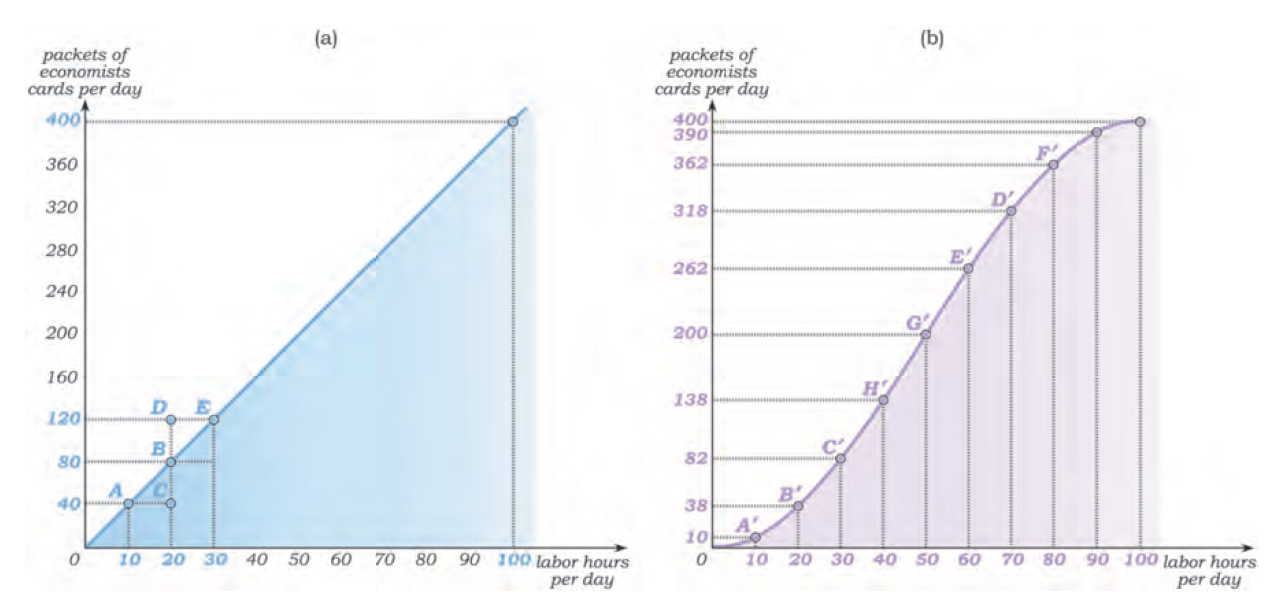
\includegraphics[width=1\textwidth]{11_1} %插入图片,[]中设置图片大小,{}中是图片文件名
	\caption{Two Types of Producer Choice Sets and Associated Production Frontiers} %最终文档中希望显示的图片标题
	\label{Fig.main2} %用于文内引用的标签
\end{figure}

\subsection{对利润的“偏好”}
等利润线:生产者的无差异曲线
\begin{figure}[H] %H为当前位置,!htb为忽略美学标准,htbp为浮动图形
	\centering %图片居中
	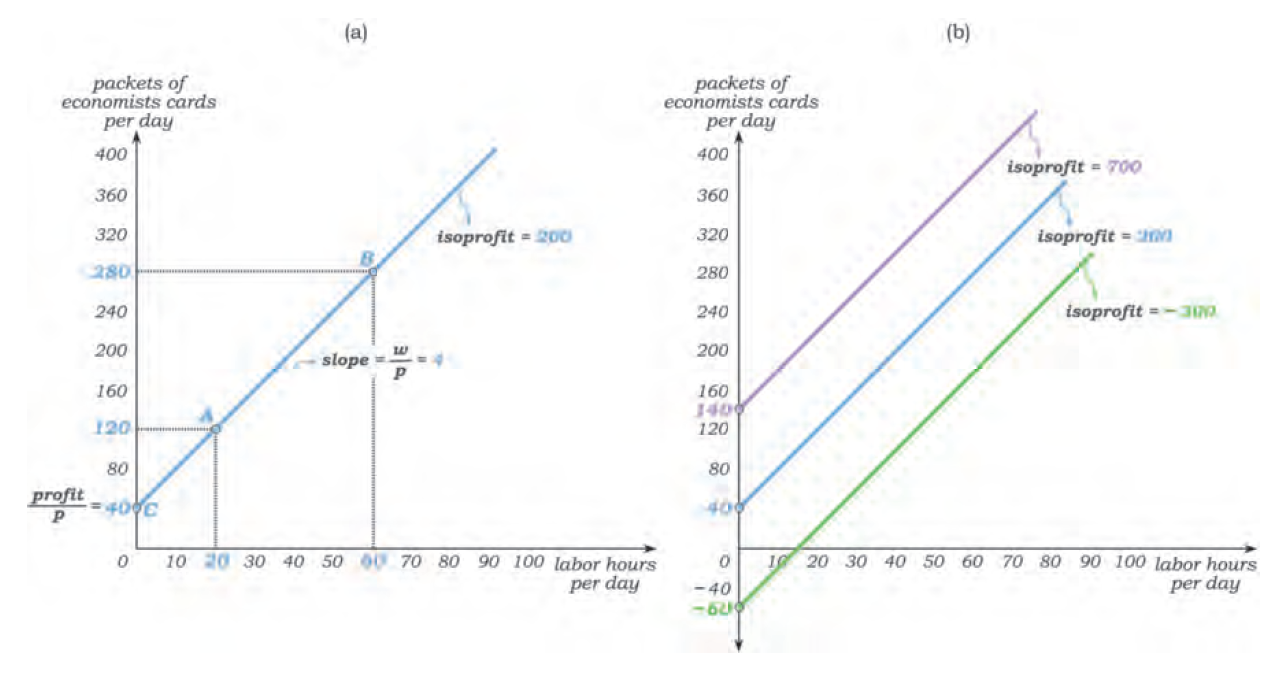
\includegraphics[width=1\textwidth]{11_2} %插入图片,[]中设置图片大小,{}中是图片文件名
	\caption{Producer Indifference—or Isoprofit—Curves} %最终文档中希望显示的图片标题
	\label{Fig.main3} %用于文内引用的标签
\end{figure}

等利润线的斜率是w/p,对生产者来说,工资和价格固定时所有等利润线都有相同的斜率。另一方面,纵截距仅仅是与等利润线相关的利润除以产出的价格。

在消费者模型中,价格影响消费者选择集的大小和形状,尤其是它还能决定预算约束的斜率。但是价格对消费者偏好和表示消费者偏好的无差异曲线没有任何影响。

在生产者模型中,事情恰好相反。价格对于生产者选择集没有任何影响,但是对于无差异曲线或等利润线的形状却有很大影响。

生产者选择集的大小和形状是由技术决定的。

另一方面,生产者的无差异曲线完全是由经济中的价格决定的,无差异曲线的截距由价格决定,斜率由工资和价格共同决定。

\subsection{选择最大化利润的生产计划}

MP(边际产品)=w/p

\begin{figure}[H] %H为当前位置,!htb为忽略美学标准,htbp为浮动图形
	\centering %图片居中
	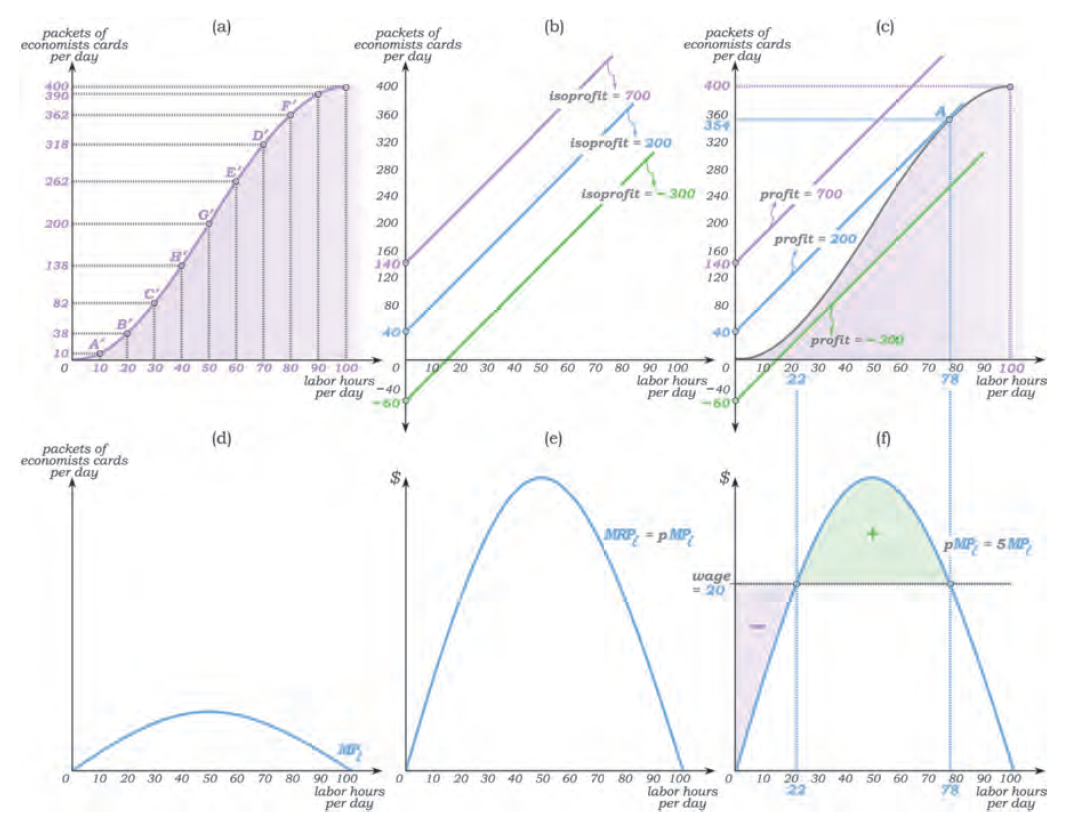
\includegraphics[width=1\textwidth]{11_3} %插入图片,[]中设置图片大小,{}中是图片文件名
	\caption{Maximizing Profit} %最终文档中希望显示的图片标题
	\label{Fig.main4} %用于文内引用的标签
\end{figure}

\subsection{改变经济环境}
市场工资的改变:
\begin{figure}[H] %H为当前位置,!htb为忽略美学标准,htbp为浮动图形
	\centering %图片居中
	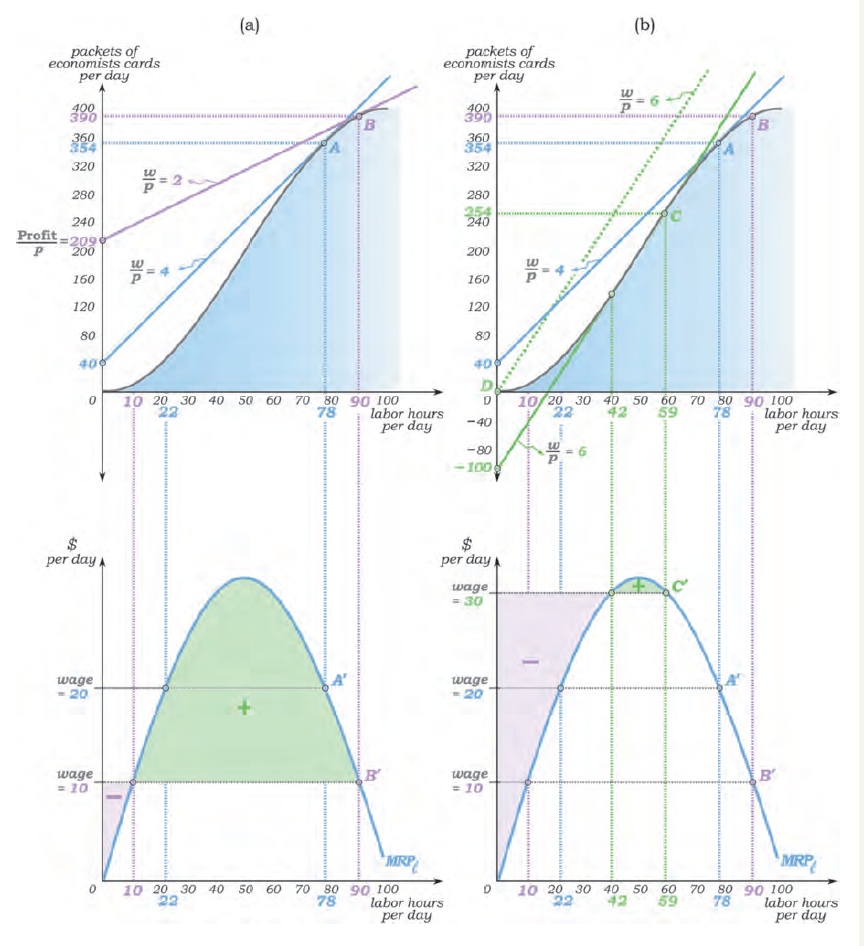
\includegraphics[width=1\textwidth]{11_4} %插入图片,[]中设置图片大小,{}中是图片文件名
	\caption{The Impact of Changing Wages on Profit-Maximizing Choices} %最终文档中希望显示的图片标题
	\label{Fig.main5} %用于文内引用的标签
\end{figure}

劳动需求曲线:表示在不同市场水平下生产者将雇佣的工时数的曲线:

\begin{figure}[H] %H为当前位置,!htb为忽略美学标准,htbp为浮动图形
	\centering %图片居中
	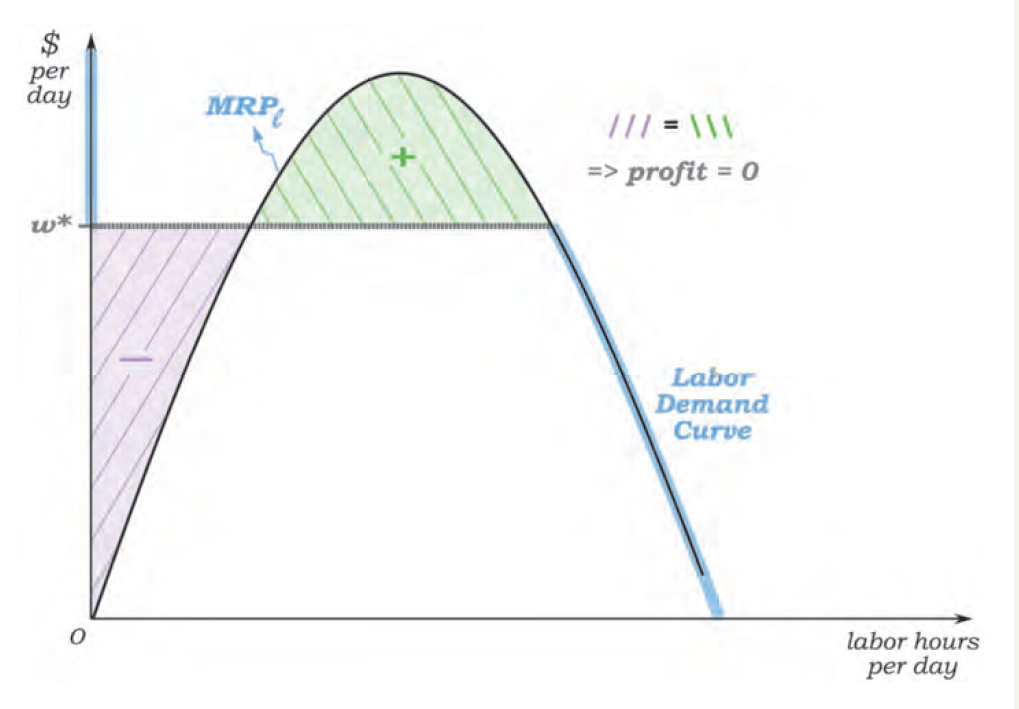
\includegraphics[width=1\textwidth]{11_5} %插入图片,[]中设置图片大小,{}中是图片文件名
	\caption{MRP and Labor Demand} %最终文档中希望显示的图片标题
	\label{Fig.main6} %用于文内引用的标签
\end{figure}

当市场工资不高于$ w^* $时,生产者将沿着MRP下降的部分雇佣工人;当市场工资高于$ w^* $时,生产者将不会雇佣任何工人。

\hspace*{\fill}

产出价格的变化:当产出价格变化时,MRP曲线本身会放缩。

\begin{figure}[H] %H为当前位置,!htb为忽略美学标准,htbp为浮动图形
	\centering %图片居中
	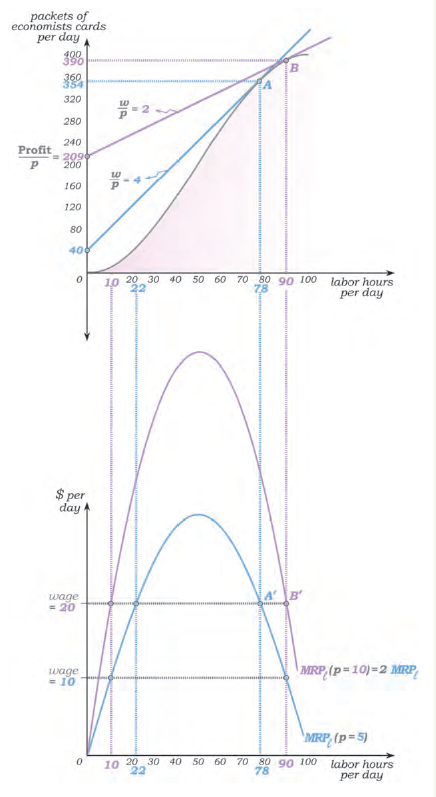
\includegraphics[width=0.7\textwidth]{11_6} %插入图片,[]中设置图片大小,{}中是图片文件名
	\caption{The Impact of Changing Prices on Profit-Maximizing Choices} %最终文档中希望显示的图片标题
	\label{Fig.main7} %用于文内引用的标签
\end{figure}

\hspace*{\fill}

产出供给曲线

\begin{figure}[H] %H为当前位置,!htb为忽略美学标准,htbp为浮动图形
	\centering %图片居中
	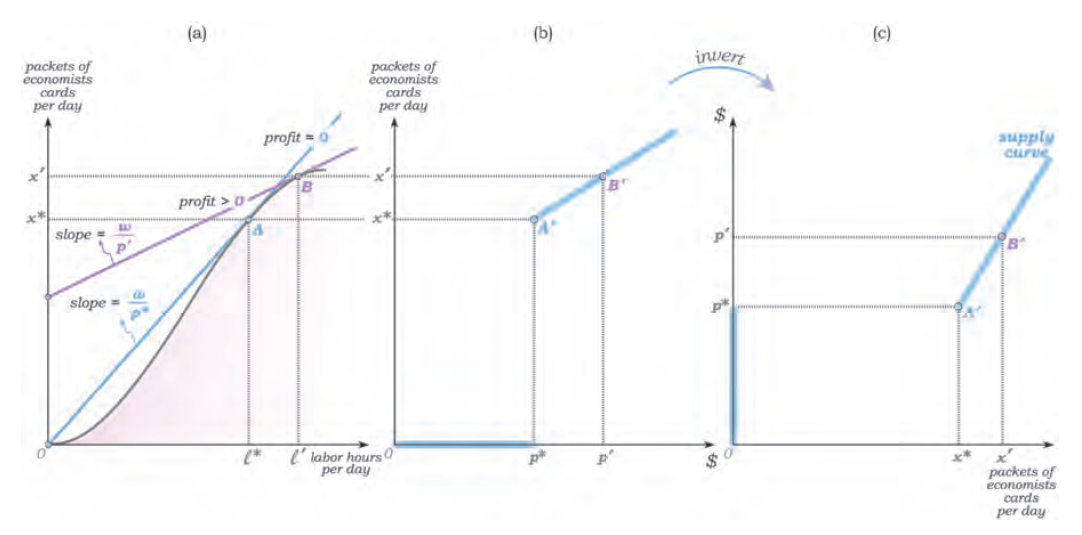
\includegraphics[width=1\textwidth]{11_7} %插入图片,[]中设置图片大小,{}中是图片文件名
	\caption{The Output Supply Curve} %最终文档中希望显示的图片标题
	\label{Fig.main8} %用于文内引用的标签
\end{figure}

当产出价格下降到$ p^* $以下时,工厂将停产。

\subsection{在利润最大化的过程中成本最小化}

利润最大化问题可以分解为两方面:

第一,我们仅仅思考当公司生产任意产量时将产生多大成本。这将使我们基于投入价格而非产出价格衍生出成本曲线;

第二,应该生产多少产量使得收益(在市场上出售产品)与成本之差最大化。

\begin{figure}[H] %H为当前位置,!htb为忽略美学标准,htbp为浮动图形
	\centering %图片居中
	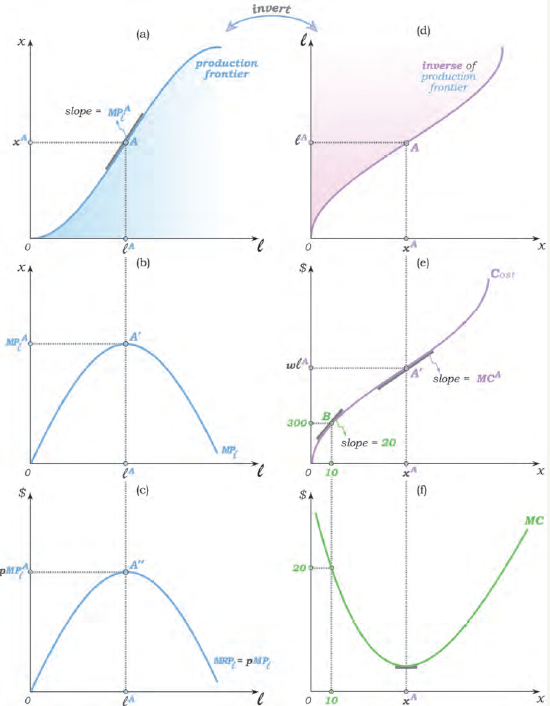
\includegraphics[width=1\textwidth]{11_8} %插入图片,[]中设置图片大小,{}中是图片文件名
	\caption{Deriving Total and Marginal Cost from Production Frontiers} %最终文档中希望显示的图片标题
	\label{Fig.main9} %用于文内引用的标签
\end{figure}

利润最大化存在条件:边际成本递增。

成本曲线上的利润最大化:给定我的由生产边界描述的生产技术以及给定工资水平w,就可以推出MC曲线。

\begin{figure}[H] %H为当前位置,!htb为忽略美学标准,htbp为浮动图形
	\centering %图片居中
	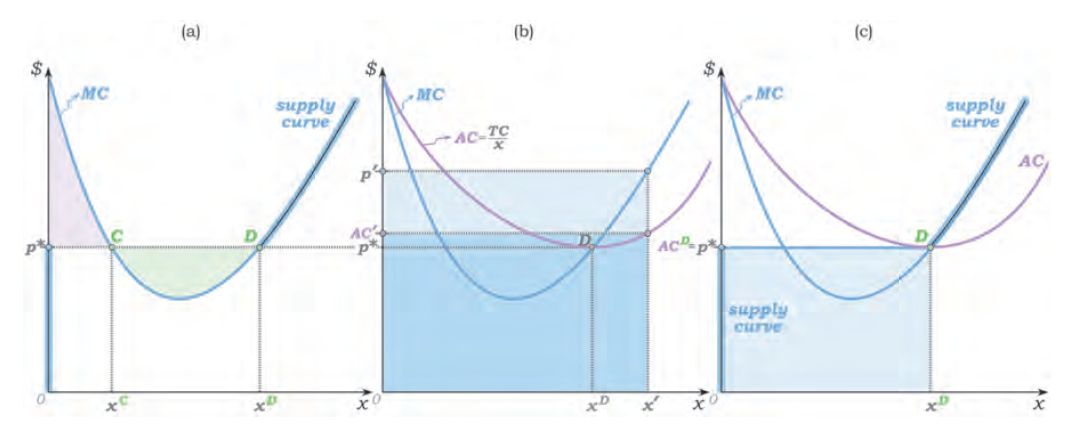
\includegraphics[width=1\textwidth]{11_9} %插入图片,[]中设置图片大小,{}中是图片文件名
	\caption{Deriving the Output Supply Curve from MC} %最终文档中希望显示的图片标题
	\label{Fig.main10} %用于文内引用的标签
\end{figure}

AC曲线与MC曲线的逻辑关系更为清晰;首先,两条曲线开始的纵轴截距是一样的;其次当边际成本曲线穿过AC曲线时,AC曲线达到其最低点。

\section{短期模型的数学分析}
\subsection{生产者面临的技术约束}

生产者计划、生产者选择集和生产边界
由生产函数$ f:\mathbb{R}^1_+\rightarrow\mathbb{R}^1_+ $定义的生产者选择集C可写为
\[
C( f:\mathbb{R}^1_+\rightarrow\mathbb{R}^1_+)=\{(x,l)\in\mathbb{R}^2|x\le f(l)\}
\]

劳动的边际产品:
\[
MP_l=\frac{df}{dl}
\]

递减的劳动边际产品
\[
\frac{dMP_l}{dl}=\frac{d^2f}{dl^2}<0
\]

\subsection{对利润的偏好}

当产出价格为p,工资率是w时,等利润线P定义为:

\[
P(\pi,w,p)=\{(x,l)\in\mathbb{R}^2|\pi=px-wl\}
\]

\subsection{选择利润最大化的生产计划}

建立生产者最优化问题:

\[
\max\limits_{x,l}=px-wl\quad s.t.\quad x=f(l)
\]

1. 把约束代入目标函数;2. 建立拉格朗日函数;3. MP=w/p

\subsection{劳动需求、产出供给与“真正最优”}

解决最优化的方法隐式定义了劳动需求函数,即对任意工资率和价格p给出了劳动需求量:
\[
l=l(p,w)
\]

一旦有了对于每个产出价格和工资率将会雇佣多少工时的函数$ l(p,w) $时,可以很快地推出产出供给函数
\[
x(p,w)=f(l(p,w))
\]

根据产出供给和劳动需求函数表达式,可以推导出利润函数:
\[
\pi=\pi(p,w)=px(w,p)-wl(p,w)
\]

\hspace*{\fill}

在确定某个特别的生产计划式利润最大化的之前,应该仔细检查以确保该生产计划的利润不为负。利润为负是应停工。

只要真正的利润最大化计划不在生产者选择集的角点,一阶条件就是生产者达到利润最大化的必要条件。角点解一般有两个:1.生产为零;2.生产无限。

\subsection{利润最大化过程中的成本最小化}

运用f(x)的反函数:
\[
l(x)=f^{-1}(x)
\]
简单地将其乘以劳动成本w得到函数
\[
C(w,x)=wl(x)
\]

生产必须满足的约束:

\[
p=MC(w,x)\enspace if\enspace p\ge \min_{x}{AC(w,x)}
\]

因此供给函数$ x(p,w) $为:
\begin{equation*}
	\begin{split}
	x(p,w)&=MC^{-1}(p,w)\enspace if\enspace p\ge \min_{x}{AC(w,x)}\\
	&=0\enspace if\enspace p<\min_{x}{AC(w,x)}
	\end{split}
\end{equation*}

MC与AC的关系:当$ AC=AC_{min} $时,MC=AC

\end{document}